\documentclass{acm_proc_article-sp}
\setlength{\paperheight}{297mm}
\setlength{\paperwidth}{210mm}

\usepackage{txfonts}
\usepackage{pifont}
\usepackage{cite}
\usepackage{graphicx}
\usepackage{url}
\usepackage{array}
\usepackage{multirow}
\usepackage{color}
\usepackage{booktabs}
\usepackage{xparse}
\usepackage{float}
\usepackage{lipsum}
\usepackage{refcheck}

\setkeys{Gin}{width=0.98\linewidth}
\graphicspath{{./figures/}}

\IfFileExists{zi4.sty}{\usepackage{zi4}}{\usepackage{inconsolata}}
\usepackage{listings}
\definecolor{bluekeywords}{rgb}{0.13,0.13,1}
\definecolor{greencomments}{rgb}{0,0.5,0}
\definecolor{redstrings}{rgb}{0.9,0,0}
\lstset{language=Java,
	xleftmargin=7mm,
	xrightmargin=2mm,
	frame=single,
	framesep=3pt,
	aboveskip=2em,
	belowskip=1em,
	numbers=left,
	numbersep=9pt,
	captionpos=b,
	tabsize=2,
	keepspaces=true,
	showspaces=false,
	showtabs=false,
	breaklines=true,
	showstringspaces=false,
	breakatwhitespace=true,
	commentstyle=\color{greencomments},
	keywordstyle=\color{bluekeywords},
	stringstyle=\color{redstrings},
	basicstyle=\ttfamily\lst@ifdisplaystyle\scriptsize\fi,
	morekeywords={
		rep,norep,owner,world,any,peer,
		where,reads,writes,pure,impure,
		intersects,disjoint,unique,lost,self},
	otherkeywords={&,?},
	escapeinside={/*@}{@*/},
	floatplacement=t
}

\usepackage{varioref}
\PassOptionsToPackage{pdfpagelabels=false}{hyperref}
\usepackage{hyperref}
\usepackage{cleveref}

\setlength{\parindent}{15pt}

\begin{document}

\title{Ownership Types for Local Reasoning}
\subtitle{CS5218: AY2014/2015 Semester 2, Final Project}

\numberofauthors{3}

\author{
\alignauthor
Darius Foo\\
		\affaddr{A0097282@u.nus.edu}
\alignauthor
Daryl Seah\\
		\affaddr{A0026468@u.nus.edu}
\alignauthor
Joel Low\\
		\affaddr{A0097630@u.nus.edu}
}



\maketitle
\begin{abstract}
The use of ownership types improves local reasoning, allowing both programmers
and program analysis tools to reason more comprehensively about the correctness
and behaviour of programs. This would improve the scalability of program
analysis tools. This paper examines five variations of ownership types, and
compares their expressiveness as well as their ability to achieve the goal of
improving local reasoning. However, owing to the difficulty of annotating
programs, it is likely that ownership types will only be used in
safety-critical programs.
\end{abstract}

\section{Introduction}
\label{sec:introduction}

The advent of Object-Oriented Programming has allowed programmers to write and
maintain larger components and programs, owing to the modularisation brought
about by encapsulation. This increased modularisation of programs ought to
result in a corresponding ease of comprehension for programmers, since
programmers are now able to reason about programs at a modular level.
Likewise, it should follow that static program analysis tools be able to
improve the speed at which analyses can be completed, especially when analysing
a large program.

In practice, many escape mechanisms which break the encapsulation of an object
are used. These mechanisms, while allowing expressiveness in programs, prevent
the programmer from reaping the benefits of being able to isolate a module and
reason about its behaviour and effects. We present an example in
\cref{code:modular_reasoning_car_engine_1}, originally
described in~\cite{clarke98ownership}.

\lstinputlisting[
	float,
	caption={Car}, 
	label=code:modular_reasoning_car_engine_1
]{examples/motivation/1.java}

Here we present a car with a driver and an engine. The car defines a
\lstinline|start| method which will start the engine, but only if a driver is
present. However, due to the lack of encapsulation, the car's engine can be
started directly in \cref{code:modular_reasoning_car_engine_1_engine_start},
bypassing the check. This should not be allowed because it breaks
encapsulation.

The traditional means of preventing this is to utilise access specifiers: using
Java's syntax, there would be four levels of access: \lstinline|public|,
\lstinline|protected|, \lstinline|private|, and default (package-level) access.
These access specifiers are annotations on types and variables, limiting
\emph{visibility} of the identifiers of said types and variables to the
appropriate scope. \Cref{code:modular_reasoning_car_engine_2}, modified from
\cref{code:modular_reasoning_car_engine_1}, demonstrates their use, but also
that enforcing encapsulation using access specifiers alone is insufficient.

\lstinputlisting[
	float,
	caption={Car with Access Specifiers},
	label=code:modular_reasoning_car_engine_2
]{examples/motivation/2.java}

In \cref{code:modular_reasoning_car_engine_2} we annotate each method
and member variable with an appropriate access specifier. We also define an
additional \emph{accessor} method, for the situation where a property of the
car's engine must be accessed outside of the car (such as an instrument
attached to the car's electronics to measure performance.) However, as seen on
\cref{code:modular_reasoning_car_engine_2_engine_start}, the original
problem has not been resolved: the engine can still be started externally.
There is no way to reconcile access to parts of an object based on who `owns'
the object, and who is accessing the object. Thus, access specifiers alone are
not expressive enough.

While access specifiers can be modified to support such a
scenario\footnote{Read-only and mutable interfaces can be extracted from the
class, and the appropriate interface returned from methods. This is not common
practice; however, the Cocoa runtime for Objective-C is notable for doing
this.}, the resulting API is clumsy because every time a type is defined,
programmers must manually define the behaviours allowed by mutable and
immutable references to the object. There would consequently be an explosion of
types, making reasoning about the program more difficult.

In this report, we describe and evaluate how ownership types can be leveraged
for local reasoning in the analysis and verification of programs.
\Cref{sec:ownership} provides an introduction to concept of ownership types,
the core principles and terminology used, and its various applications in
program analysis. \Cref{sec:systems} gives a detailed overview of each of the
four ownership type systems that we have investigated in depth. \Cref{sec:eval}
provides a comparative evaluation on the expressiveness of each system and
their benefits for local reasoning and analysis. Finally, we conclude in
\cref{sec:conclusion} with a summary of the fundamental limitations of
ownership types. Our coverage of the topic in breadth is spread over
\cref{sec:ownership,sec:systems}.


\section{Ownership Types}
\label{sec:ownership}

% terminology and the basics
Ownership Types enhance the type system by allowing ownership information to be
stored together with type information; this directly overcomes the limitations
of only using access specifiers. Using SafeJava's~\cite{boyapati04safejava}
syntax, the Car example can be expressed as per
\cref{code:ownership_types_car_engine_1}
\vpageref[above]{code:ownership_types_car_engine_1}.

\Cref{code:ownership_types_car_engine_1} introduces the notion of an ownership
\emph{type}. Just like generics, this is information which is created and
enforced statically. All types are now parameterised by an ownership type,
preventing objects with different owners from being assigned (and indeed,
referenced). Furthermore, it is not possible to express the ownership type of
an object belonging to another object, preventing the encapsulation violation
on \cref{code:ownership_types_car_engine_1_engine_start}.

\lstinputlisting[
	float,
	caption={Car with Ownership Types},
	label=code:ownership_types_car_engine_1
]{examples/motivation/3.java}

Ownership parameters can also be used within the class declaration, as shown on
\cref{code:ownership_types_car_engine_1_parametric_owner}. Special keywords
have been introduced: \lstinline|world| indicating that the value is not owned
by any object (i.e. it is owned by the system), and \lstinline|this| has been
overloaded to refer to the current object's ownership context.

Type-checking this program results in a type-check failure because it is not
possible to express the ownership context of the car outside of the class.
However, it is possible to express the car's ownership of objects used by it
through the ownership parameter mechanism.

This is one of the few approaches that we have examined. The other approaches
are conceptually similar; the difference among them lies mainly in their
expressivity.

\subsection{Definitions}
\label{subsec:definitions}

In this paper, we try to make our definitions as generic as possible, allowing
a consistent set of terms to be used across the different systems proposed.

\begin{description}
	\item[Expressivity] How complex a notion of ownership a system can allow a
		programmer to express. We have designed various use cases which
		encompass a variety of design patterns found in programs used today, and
		analysed each system for its ability to express such a design pattern.
		Our use cases can be broadly categorised as such:

	\begin{itemize}
		\item \textbf{Abstract Data Types}: We modified a Queue example
			from~\cite{boyapati04safejava} and added iterators, which can be
			seen as a view over the data stored in the data type.
		\item \textbf{Inheritance}: A recurring pattern in Object-Oriented
			Programming where new classes are augmented with behaviour from
			existing classes.
		\item \textbf{Generics}: Building upon the ADT use case, Generics
			allow programmers to take advantage of parametric polymorphism to
			write reusable components.
		\item \textbf{Cardinality of Ownership}: Having multiple owners for an
			object is useful for writing parallel/distributed algorithms.
		\item \textbf{Ownership Transfer}: Allowing the transfer of ownership
			from one object to another is useful in the \linebreak
			producer-consumer pattern.
	\end{itemize}

	\item[Representation Invariant] A constraint on the state of an object,
		maintained throughout its lifetime.
	\item[Owner] An object or set of objects responsible for maintaining the
		representation invariant of an object.
	\item[Context \emph{a.k.a. Universe, Box}] A nested partition of the object
		store containing all the objects constituting the representation of
		a particular object.
\end{description}

\subsection{Ownership Topologies}
\label{subsec:topologies}

An ownership topology describes the structure and organisation of the
object store. In this paper, two topologies are examined:

\begin{description}
	\item[Hierarchical \emph{a.k.a. Tree}] This is a single ownership topology,
		\linebreak where every object as one owner.
	\item[Directed Acyclic Graph (DAG)] This is a multiple ownership \linebreak
		topology, where an object can have multiple owners. All owners of the
		object can modify its invariant.
\end{description}

\subsection{Encapsulation Disciplines}
\label{subsec:encapsulation}

Where an ownership topology \emph{describes} the structure of the object store,
an encapsulation discipline \emph{prescribes} the structure of the object
store. They can thus be seen as related ideas. In this paper, two main
encapsulation disciplines are discussed:

\begin{description}
	\item[Owners-as-Dominators] Objects can only be modified by following a
		reference chain from the root context through the object's owner.
		Aliasing is restricted, because no aliases to an object B owned by an
		object A can exist outside of the ownership context of object A.
	\item[Owners-as-Modifiers] Objects can only be modified by following a
		reference chain from the root context through the object's owner.
		However, read-only access is granted in all other contexts. Aliasing is
		\emph{not} restricted.
\end{description}

\begin{figure}[t]
	\centering
	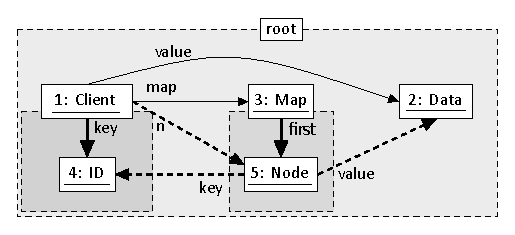
\includegraphics{ownership-dominator-vs-modifier.eps}
	\caption{Owners-as-Dominators vs. Owners-as-Modifiers}
	\label{fig:ownership-dominator-vs-modifier}
\end{figure}

\Cref{fig:ownership-dominator-vs-modifier} (taken from~\cite{dietl09gut})
illustrates the difference between both encapsulation disciplines. References
between objects are represented by arrows. The owner of an object is the class
at the top of the dashed box the object is in.

If the \textbf{owners-as-dominators} discipline is adhered to, then \linebreak
only the solid arrows are allowed. The dashed arrows are references which do
not pass through the object's owner, and as such are only allowed in the
\textbf{owners-as-modifiers} discipline. In the \textbf{owners-as-modifiers}
discipline, while such a reference is legal, these references cannot be used to
mutate the state of the object being referenced.

\subsection{Applications}
\label{subsec:applications}

\subsubsection{Object Encapsulation}
\label{subsubsec:object_encapsulation}

Deriving directly from the example problem given in our
\hyperref[code:modular_reasoning_car_engine_1]{introduction}, ownership types
can be used to improve the expressibility of the concept of
ownership~\cite{clarke98ownership}. This allows classes to restrict
modification of their representation invariants by external code.

Therefore, when programmers are given a new code base annotated with ownership
types, they can be ensured that no external code is able to modify the classes'
invariants when they are understanding the code. This would allow them to
locally reason about the function and behaviour of the module.

The same benefit would also apply for static analysis tools. Because changes can
be effected only from one part of the program, a tool need only reason locally
to form sound conclusions. This would allow such tools to run in parallel on
different parts of the program, allowing even complex analyses to scale with the
size of the code base.

\subsubsection{Alias/Access Control}
\label{subsubsec:alias_control}

If programs adhere to the \textbf{owners-as-dominators} encapsulation
discipline, then it is not possible to reference objects within another
object's representation. Therefore, aliases would be restricted to
the scopes where references are
allowed~\cite{clarke98ownership,boyapati04safejava,cameron07mojo}.

If programs adhere to the \textbf{owners-as-modifiers} encapsulation
discipline, then there is no alias control; however, it is still not possible
to modify the representation of an object if the current object is not its
owner~\cite{cunningham08ut,dietl09gut}.

In both cases, reasoning about side-effects are easy. In the former case, it is
possible to increase the precision of alias analyses because aliasing is
restricted to scopes where the reference is valid.

\subsubsection{Data Race/Deadlock Prevention}
\label{subsubsec:data_race_prevention}

Because ownership types impose a structure on the object store, it is possible
to prevent data races. Typically, when an object \textbf{A} needs to be locked
for an update, it is not obvious which dependent objects (references which
\textbf{A} maintains) need to be locked as well. Since there is an ownership
topology imposed on the object store, it would be possible to know at
compile-time which objects need to be locked as part of locking \textbf{A}.
This prevents data from being accessed if an object is left unlocked by human
error; data races can thus be prevented.

In the same vein, it is possible to prevent deadlocks from occurring by always
acquiring a set of locks in the same order. Acquiring multiple locks in the same
order prevents a circular wait condition, which is a necessary condition for a
deadlock to occur~\cite{silberschatz08os}. Regardless of topology,
locking objects using depth-first or breadth-first traversal guarantees that
all objects which are reachable will be locked. Furthermore, because the
traversal is deterministic, it is guaranteed that the order of lock acquisition
is always the same~\cite{boyapati02races}.

\subsubsection{Persisted Object Upgrades}
\label{subsubsec:object_upgrades}

Very often programs need to persist state to disk. The structure of this state
might vary between versions of the same program. A problem is presented to the
programmer: how to use the data (in the old format) in the updated program?
Typically programmers will write transform functions which accept the old
program state as input, and produces the corresponding new program state. This
works well for simple objects; however, when the object graph is large, or
contains cycles, the order to execute these transform functions may not be
obvious.

Ownership types enforce constraints on the structure of the object graph. This
allows the programmer to write isolated transform functions that transforms only
one type in the object graph. When used together with a transactional memory
store, it is possible to individually transform objects in any order, so long as
all objects in the graph are eventually transformed. When the transaction is
committed, it may be statically guaranteed that the new object graph would be
valid~\cite{boyapati04safejava,boyapati03innerclass}.

\section{Ownership Type Systems}
\label{sec:systems}

% note: should be four systems. we just present UT and GUT separately in eval.
In this section we give an overview of the four ownership type systems that we
have investigated in-depth. The papers covered are by no means the entirety of
the work in the area. There are numerous other papers on extensions,
improvements and related developments~\cite{clarke13survey}. However, we chose
these systems because they contributed important ideas and are
representative of the gamut of work in ownership types. Each system will be
presented individually with a full cross-comparison provided in \cref{sec:eval}.

\subsection{Clarke's Ownership Types}
\label{subsec:clarke}

The concept of ownership was first introduced by Clarke et
al.~\cite{clarke98ownership,clarke01ownership} with the intention of
mitigating the problems of uncontrolled aliasing in Object-Oriented languages.
This was a refinement of a similar idea proposed by Clarke's thesis advisors
called \emph{flexible alias protection}~\cite{noble98alias} which, in turn,
took inspiration from Islands~\cite{hogg91islands} and
Balloons~\cite{almeida97balloons}.

Islands and Balloons were early attempts at solving the same problem but did
not provide sufficient expressivity and ease-of-use to be practical. For
example, an object cannot be stored in two fully-encapsulated containers
simultaneously since a stored object would be considered a part of the
container's island/balloon and cannot be externally aliased. To mitigate this
problem, dynamic aliases (i.e.\ temporary stack-based references) into a
representation are permitted in both these works. Such aliases are read-only in
Islands, but have no restrictions in Balloons. Thus, while this escape
mechanism solves the problem, it can also expose the representation of the
container itself (e.g.\ nodes in a link-list) and provide no encapsulation in
the case of Balloons. Moreover, the authors of~\cite{noble98alias} argue that
it would be hard for programmers to use Balloons because of the complex
abstract interpretation required.

Ownership types solve the problem by providing a more flexible/intuitive syntax
to the programmer for defining a hierarchical topology over objects without
sacrificing encapsulation. The idea is to annotate types with modifiers
that define which context (i.e.\ owner) each reference belongs to, which
include:
\begin{itemize}
	\item \textbf{\lstinline|norep|}:
		Not part of the representation of any object.
	\item \textbf{\lstinline|rep|}:
		Owned by \lstinline|this| object and is part of its representation.
	\item \textbf{\lstinline|owner|}:
		Owned by the owner of \lstinline|this| object.
	\item \textbf{$v$}:
		A context parameter.
\end{itemize}

Context parameters are declared on classes with a syntax similar to Java's
generics, e.g. \lstinline|class List<elementOwner> { ... }|, and are similarly
applied on types, e.g. \lstinline|rep List<norep> list;|. They allow owners
higher in the hierarchy to declare their ownership of references held by
descendants in their contexts. In the case of the previous \lstinline|list|
example, the \lstinline|list| is declared to be part of the client object's
context, but the elements it contains has no owner. Parameterised ownership is
the key innovation that (partially) solves the container problem and also
enables different roles for different references of the same object class.

These declarations and parameters describe a hierarchical structure of object
representations that can be easily verified at compile-time. If well-typed, the
programmer can be assured that there are no external aliases to any of the
objects within a particular context, guaranteeing encapsulation. In particular,
Clarke's ownership types enforces the \textbf{owners-as-dominators} discipline,
which ensures that all paths to an object must pass through its owner.

However, ownership types as originally presented in~\cite{clarke98ownership}
still had limitations. For example, rules for inheritance/subtyping were yet to
be developed and the encapsulation discipline was still too strict to be of
practical use (e.g.\ iterators were not possible.) Addressing these and other
limitations was the main focus of subsequent work on the subject, a few of
which are covered in the following sections~\cite{boyapati04safejava,
boyapati03innerclass, cunningham08ut, dietl11gut, cameron07mojo}.

% Iterators not possible (too strict because of owners-as-dominators discipline)
% - In XStack example, iterator modification has to go through stack
%
% - Iterator is only usable in the context of the owner of both the iterator and
%	 stack
%
% - Boyapati: A type system that strictly enforces object encapsulation is
%	 too constraining [113]: it does not allow efficient implementation of
%	 important constructs like iterators [104, 71]. Consider, for example, an
%	 iterator over the above-mentioned Stack object s. If the iterator is
%	 encapsulated within s, it cannot be used outside s. If the iterator is not
%	 encapsulated within s, it cannot directly access the list nodes in s, and
%	 hence cannot run efficiently. [SafeJava, pg 25]
%
% Multiple owners not possible
% - Cannot append two XStacks together because an append() function would have
% to be declared rep. The other xstack would have a problem to be passed to the
% first xstack because the contexts are different
% Not possible to transfer ownership
% - Example?


\subsection{Boyapati's SafeJava}
\label{subsec:boyapati}

Boyapati et al.\ tackled the expressivity problem with the intention of making
ownership types a practical solution for local reasoning and software upgrades
in persistent object stores~\cite{boyapati03innerclass}. His idea was to simply
provide an exception for inner-classes (which iterators are often implemented
with) to directly access and manipulate the representation of their outer-class
regardless of ownership, while retaining the \textbf{owners-as-dominators}
discipline in all other cases.\footnote{Clarke actually proposed a similar idea
in his thesis~\cite{clarke03ownership} but with a discipline that is not as
useful for local reasoning~\cite{boyapati03innerclass}.}

The declarations and keywords used are also slightly different, but are no less
expressive than Clarke's. The first context parameter of a type is taken to be
primary owner, eliminating the need for separate \lstinline|norep|,
\lstinline|rep| or \lstinline|owner| modifiers and making the syntax more
consistent. Context arguments can be one of the following:
\begin{itemize}
	\item \textbf{\lstinline|this|}:
		Referencing \lstinline|this| object as the owner.
	\item \textbf{\lstinline|world|}:
		Referencing the root context as the owner.
	\item \textbf{$v$}:
		A parameterised owner.
\end{itemize}

For example, the \lstinline|list| in \cref{subsec:clarke} would be declared
as\linebreak\lstinline|class List<listOwner, elementOwner> { ... }|
and\linebreak\lstinline|List<this, world> list;|~~in Boyapati's syntax.

Boyapati eventually developed his version of ownership types into a system
called SafeJava~\cite{boyapati04safejava} with additional features supporting
not just software upgrades and local reasoning but also data race/deadlock
prevention and region-based memory. These include:
\begin{itemize}
	\item \textbf{Inheritance} and subtyping rules for ownership.
	\item \textbf{Constraints} on classes and methods with \lstinline|where|
clauses,\linebreak e.g.~~\lstinline|class Container<o, a, b, c, d> where b <= c { /* b must be identical to or an ancestor of c */ }|.
	\item \textbf{Effects} clauses with the \lstinline|reads| and
\lstinline|writes| keywords declaring which variables are read and written by a
method.
	\item \textbf{Transfer} of ownership from one context to another, enabled by
declaring such references to be \lstinline|unique|.
\end{itemize}

While impressive overall, we find that the ``principled violation of
encapsulation'' as the authors call it) for inner-classes is not a particularly
elegant solution.\footnote{In fact, Aldrich and Chambers have generalized such
an approach in their development of \emph{ownership
domains}~\cite{aldrich04domains}. We did not have time to evaluate this system
in depth, but it appears to be \emph{too} expressive for programmers to use
easily in practice.} Moreover, binary operations such as
\linebreak\lstinline|list1.addAll(list2)| and other patterns are also still
problematic to express in both Clarke's and Boyapati's systems.

% - Boyapati: A type system that strictly enforces object encapsulation is
%	 too constraining [113]: it does not allow efficient implementation of
%	 important constructs like iterators [104, 71]. Consider, for example, an
%	 iterator over the above-mentioned Stack object s. If the iterator is
%	 encapsulated within s, it cannot be used outside s. If the iterator is not
%	 encapsulated within s, it cannot directly access the list nodes in s, and
%	 hence cannot run efficiently. [SafeJava, pg 25]

%
% - Ownership types can be mostly verified at compile time, but dynamic casts
% are allowed in Java and so he proposes a complementary runtime system that
% checks casts.

\subsection{Dietl and M\"{u}ller's Universe Types}
\label{subsec:dietl}

Universe Types~\cite{cunningham08ut} is an ownership system that takes a
somewhat different approach to the problem. Influenced by Clarke's original
work on ownership~\cite{clarke98ownership} and M\"{u}ller's concept of
Universes~\cite{muller99universes}, Dietl et al.\ developed Universe Types for
the purpose of local reasoning in program verification~\cite{cunningham08ut,
dietl09gut, dietl11gut}.

Their key insight is that restricting aliasing is not really necessary for
program verification --- it is sufficient to simply restrict the references
that may modify an object to those held by objects within the owner's
context~\cite{dietl11gut}, and permit read-only access in all other cases. In
other words, to enforce the \textbf{owners-as-modifiers} discipline instead of
owners-as-dominators, thereby giving programmers greater expressibility. For
example, read-only iterators and binary operations are not an issue in Universe
Types.\footnote{Mutable iterators are still a problem.}

Instead of the fully context parametric approach of
Boyapati~\cite{boyapati04safejava}, which Clarke also
adopted~\cite{clarke03ownership}, Dietl et al.\ proposed using type modifiers
exclusively for the declaration of ownership. There are three
programmer-expressible modifiers in Universe Types: \newpage
\begin{itemize}
	\item \textbf{\lstinline|any|}:
		No restrictions on the owner. Similar to Clarke's \lstinline|norep|.
	\item \textbf{\lstinline|rep|}:
		Owned by \lstinline|this| object and is part of its representation.
	\item \textbf{\lstinline|peer|}:
		Owned by the owner of \lstinline|this| object. Similar to Clarke's
		\lstinline|owner|.
\end{itemize}

In addition, there are two non-expressible modifiers that are required for
type-checking:
\begin{itemize}
	\item \textbf{\lstinline|lost|}:
		There are constraints on the owner that cannot be expressed, i.e.\ the
		identity of the owner has been lost.
	\item \textbf{\lstinline|self|}:
		Refers to \lstinline|this| object, which is a specialisation of
		\lstinline|peer|.
\end{itemize}

\begin{figure}[t]
\centering
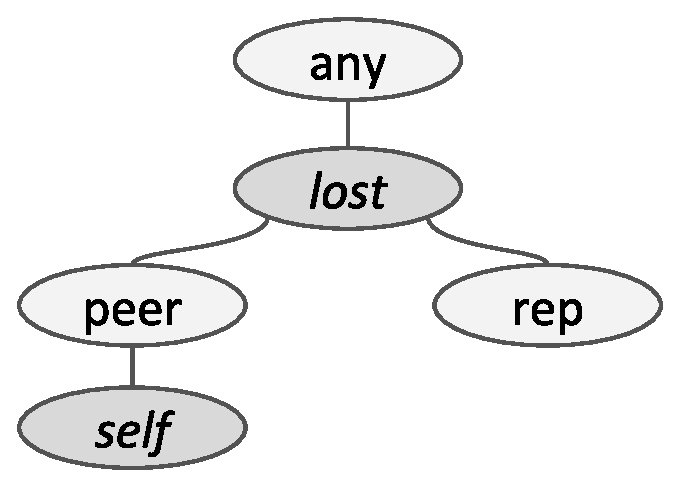
\includegraphics[width=0.5\linewidth]{ut-modifiers.eps}
\caption{Ordering of Modifiers in Universe Types.}
\label{fig:ut-modifiers}
\end{figure}

The modifier \lstinline|lost| can be the result of following a reference chain
and attempting to adapt the declared modifiers of the references to the
viewpoint of the current object. For example, following a 2-reference chain
declared \lstinline|any.rep| would result in \lstinline|lost| because
\lstinline|rep| requires a specific owner to type-check but the ownership of
its parent object is not available.

These five modifiers form a hierarchy as shown in \cref{fig:ut-modifiers}. An
object assignment (e.g.\ $\alpha$\lstinline| = |$\beta$) is legal if the
ownership type of $\alpha$ is expressible and is identical to or a
generalization of the type of $\beta$. Note that nothing can be assigned to a
\lstinline|lost| reference since the ownership information required for
verification is missing, but we can assign anything to \lstinline|any|
(including \lstinline|lost|) since the ownership information will ultimately be
discarded.

An effects system in the form of \textbf{\lstinline|pure|} and
\textbf{\lstinline|impure|} annotations on methods is also supported. Methods
are declared \lstinline|pure| if they have no side-effects (i.e.\ do not change
the state of the heap) and \lstinline|impure| otherwise. This is necessary
since external aliases to an encapsulated object are read-only and therefore
only \lstinline|pure| methods may be invoked on such references.

\lstinputlisting[
	float,
	caption={Usage of Generic Universe Types},
	label=code:usage_gut
]{examples/universe-types/generic-universe-types.java}

Universe Types is clearly limited without some form of ownership
parameterisation similar to Clarke's~\cite{clarke03ownership} and
Boyapati's~\cite{boyapati04safejava}. However, when Clarke and Boyapati
developed their ownership systems, Java had yet to introduce generic classes.
Dietl et al.\ subsequently developed Generic Universe
Types~\cite{dietl07gut,dietl09gut,dietl11gut}, which extended Universe Types to
languages that have a generic type syntax similar to Java's. As it turns out,
unlike~\cite{clarke03ownership} and~\cite{boyapati04safejava}, which conflict
with the syntax of Java's generic classes, the approach taken with Universe
Types (in applying modifiers to existing types) extends naturally to the
generic type syntax of Java and adds the ownership parameterisation necessary
to make the system practical. An example of the ownership declarations for an
imaginary set of generic collection classes (adapted from~\cite{dietl07gut}) is
provided in \cref{code:usage_gut}.

Generic Universe Types does have limitations, but it seems to be one of the more
popular and practical ownership systems in existence, likely due to its natural
compatibility with the current syntax of Java and (relative) simplicity.
Universe Types has been extended with ownership
transfers~\cite{muller07transfer}, and both Universe Types and Generic Universe
types feature type inference~\cite{dietl11inference}. Furthermore, at least two
implementations of a type checker~\cite{cameron10gut,dietl14checker} and one for
inference~\cite{dietl14checker} are available as well.

%
% Vanilla Universe Types requires runtime checking without parameterization. An
% example is the use of any for references to values in a container class. This
% implies that the references are read-only --- the user of a container cannot
% obtain and modify the objects with these read-only references UNLESS they are
% casted to rep something, with the appropriate runtime check. Generic Universe
% Types solves this problem.
%
% Iterators can be more efficient because they can have direct access to the
% representation of the container for reading and writing.


\subsection{Cameron's Multiple Ownership}
\label{subsec:cameron}

The previous type systems impose rigid object topologies well, but suffer in
expressivity: the hierarchical model of ownership cannot accommodate certain
object structures. For example, \cref{code:ownership_types_multiple}
(visualised in \cref{fig:multiple-ownership}), which is originally described
in~\cite{cameron07mojo}, is impossible to express.

\begin{figure}[t]
\centering
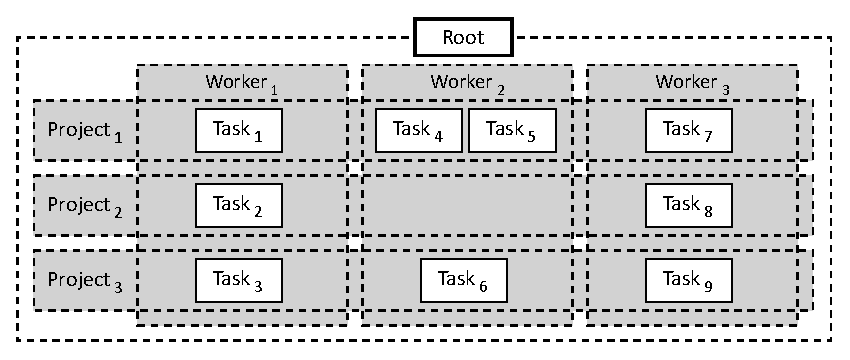
\includegraphics{multiple-ownership.eps}
\caption{Multiple Ownership}
\label{fig:multiple-ownership}
\end{figure}

The object topology presented here is a DAG instead of a tree: both Projects and
Workers may conceptually own Tasks and accordingly modify them. In other words,
the axis of organisation is flexible and may be either organised by Projects or
by Workers.

The \textbf{owners-as-dominators} discipline prevents this, as it requires that
the object topology be a tree: only one owner may dominate access paths to
Tasks. The \textbf{owners-as-modifiers} discipline also causes problems as
previously described: only either Projects or Workers may own tasks, so only
one would be able to modify them.

\lstinputlisting[
	float,
	caption={Multiple ownership},
	label=code:ownership_types_multiple
]{examples/multiple-ownership/multiple-ownership.java}

To work around this problem with single ownership, the object structure would
have to be flattened, making all the objects involved peers of each other. This
would solve the immediate problem, but would remove all encapsulation and
defeats the purpose of having an ownership type system in the first place.

These deficiencies motivated \cite{cameron07mojo}, which generalises the notion
of single ownership by reimagining ownership contexts (called boxes in their
terminology) as sets; multiple or joint ownership is then easily expressible via
set intersection.

The \textbf{owners-as-dominators} discipline is too constraining as there are
multiple access paths to objects -- it is therefore relaxed. The
\textbf{owners-as-modifiers} discipline still applies, allowing any one
of an object's multiple owners to modify it. Multiple ownership is reified with
several syntactic additions:

\begin{itemize}

	\item \textbf{Ownership parameters} (as in \cite{boyapati04safejava}), are
		used to express secondary or child owners.

	\item \textbf{An intersection operator} (\lstinline|&|) on ownership
		contexts is introduced. It specifies that an object's owner is the
		intersection of two existing ownership contexts: conceptually, if an
		object's owner is \lstinline|a & b|, it means that the object is jointly
		owned by a and b.

	\item \textbf{Wildcards} (or \textit{existential owners}) allow programmers
		to express the notion of co-owners which the current scope does not
		have access to. This is illustrated in
		\cref{code:ownership_types_multiple_wildcards}.\footnote{Ownership
		parameters as specified in the paper \textit{are} covariant; a
		notable difference from Java's generic type parameters.\linebreak
		\lstinline|Task<a & b>| is considered a subtype of both
		\lstinline|Task<a & ?>| and \lstinline|Task<b & ?>|, allowing it to be
		used wherever the latter two are expected.}

		\lstinputlisting[
			float,
			caption={Existential owners},
			label=code:ownership_types_multiple_wildcards
		]{examples/multiple-ownership/existential-owners.java}

\end{itemize}

The ability to specify intersection and disjointness constraints is supported
by the \textbf{\lstinline|intersects|} and \textbf{\lstinline|disjoint|}
keywords.

\begin{itemize}

	\item \lstinline{a} \textbf{\lstinline|intersects|} \lstinline{b} is
		required for \lstinline|a & b| to type-check. This forces the programmer
		to specify upfront which ownership contexts intersect, reducing the
		chance of erroneous or invalid ownership parameterisation.

	\item \lstinline{a} \textbf{\lstinline|disjoint|} \lstinline{b} guarantees
		effect-independence between \lstinline{a} and \lstinline{b}. This can be
		seen intuitively as we are sure that the ownership contexts of a and b
		do not intersect, and thus method calls on a and b cannot interfere.

	\item \textbf{\lstinline|where|} clauses enable us to constrain ownership
		parameters to classes. This is illustrated in
		\cref{code:ownership_types_multiple_constraints}: we are unable to take
		the intersections of disjoint ownership boxes, or boxes that we know
		nothing about. Another notable constraint is that disjoint boxes cannot
		be parameterised with identical elements as disjointness is irreflexive.

\end{itemize}

\lstinputlisting[
	float,
	caption={Multiple Ownership Constraints},
	label=code:ownership_types_multiple_constraints
]{examples/multiple-ownership/ownership-constraints.java}

Multiple ownership as described is a powerful notion but has a number of
limitations:

\begin{itemize}

	\item \textbf{The owners-as-dominators discipline is dropped}. Access paths
		are no longer restricted to one dominating object, and thus the type
		system cannot make guarantees about object encapsulation that are nearly
		% TODO: Darius please annotate this with the citation
		as strong. Cameron et al. propose future work on extending
		owners-as-dominators to accommodate multiple owners, ensuring that at
		least \textit{one of the owners} of an object dominates access paths to
		it.

	\item \textbf{Ease of use may suffer}. Ownership constraints reflect their
		implementation, which in this case is in the form of sets. Their
		semantics are difficult to reason about without a working understanding
		of the view of ownership contexts as sets, and may not be as easy to use
		as the other type systems.

	\item \textbf{Multiple ownership has not been fully generalised} to solve
		other problems that ownership types are known for, or already have
		solutions for. More specifically, work on integrating it with generics
		and race detection is ongoing. This is understandable as it is work in
		a new direction, being the first implementation to relax the
		\textbf{Owners-as-Dominators} discipline and admit multiple owners.

\end{itemize}

\section{Evaluation}
\label{sec:eval}

\begin{table*}[t]
\caption{Expressivity and (Analytical) Benefits of Ownership Type Systems}
\label{tab:summary}
\centering
\NewDocumentCommand{\rot}
	{O{45} O{1.8em} m}{\makebox[#2][l]{\rotatebox{#1}{#3}}}
\newcommand{\Yes}{$~\medbullet$}
\newcommand{\Limited}{$~\medcirc$}
\newcommand{\Maybe}{$~\bigtriangleup$}
\newcommand{\No}{$~\times$}
\newcommand{\note}[1]{\textsuperscript{$#1$}}
\newcommand{\comment}[2]{
	& & \multicolumn{12}{l}{
		\scriptsize \note{#1}\,#2 \vspace{-0.7em}
	} \\
}
\renewcommand{\arraystretch}{1.4}
\vspace{1em}
\begin{tabular}{rllllllllllllll}
	\scriptsize
	\begin{tabular}[b]{|rl|} \hline
		\Yes & Supported \\
		\Limited & Partially Supported \\
		\No & Not Supported \\
		\Maybe & Not Discussed \\
		\hline \multicolumn{1}{r}{}
	\end{tabular} \hspace{10pt}
&~&
\rot{Immutable View} &
\rot{Mutable View} &
\rot{Binary Operations} &
\rot{Class Inheritance} &
\rot{Ownership Constraints} &
\rot{Ownership Transfer} &
\rot{Generic Ownership} &
\rot{Generic Types} &
\rot{Multiple Owners} &
\rot{\bf Alias Control} &
\rot{\bf Effect Specifications} &
\rot{\bf Local Reasoning} &~~
\\ \toprule
Ownership Types~\cite{clarke98ownership}&
	& \No & \No & \No & \Maybe & \No & \No & \Yes & \Maybe & \No
	& \Yes & \Maybe & \Yes
\\
SafeJava~\cite{boyapati04safejava}&
	& \Yes & \Yes & \No & \Yes & \Yes & \Yes & \Yes & \Maybe & \No
	& \Yes & \Yes & \Yes
\\
Universe Types~\cite{cunningham08ut}&
	& \Yes & \No & \Yes & \Yes & \No & \Yes & \No & \Maybe & \No
	& \No & \Limited\note{\ast} & \Yes
\\
Generic Universe Types~\cite{dietl11gut}&
	& \Yes & \No & \Yes & \Yes & \No & \Maybe & \Yes & \Yes & \No
	& \No & \Limited\note{\ast} & \Yes
\\
Multiple Ownership~\cite{cameron07mojo}&
	& \Yes & \Yes & \Yes & \Yes & \Yes & \Maybe & \Yes & \Maybe & \Yes
	& \Yes & \Yes & \Limited\note{\dagger}
\\ \bottomrule
\comment{\ast}{
	UT/GUT only supports \lstinline|pure| and \lstinline|impure|, rather than
	the more general \lstinline|reads| and \lstinline|writes| declarations.
}
\comment{\dagger}{
	The ownership wildcard \lstinline|?| limits the local reasoning possible.
}
\end{tabular}
\end{table*}

As mentioned earlier, we have chosen to measure expressivity in terms of the
design patterns and object structures that the different systems support.

Full code examples can be found in the \texttt{examples/\linebreak~comparisons}
directory. Each code example includes a standard Java implementation (called
\texttt{standard.java}), and an equivalent implementation for each of the
systems we have examined. Systems which did not allow expressing the example
would have a comment indicating so. If a system does not allow expressing a
given syntactic construct (e.g. inheritance or inner classes), then the
implementation for that system would be omitted. A summary of our findings is
listed in \cref{tab:summary}.

\subsection{Collection Views}
\label{subsec:views}

A common design pattern when designing abstract data types is to define
\emph{views}. A view is an object that presents the data in some other
container -- iterators over a container being the most common view used in
programs today. These views may allow modification of the data type that it
is associated with. Owing to its ubiquity, we have adopted it as a benchmark
for ownership types to be able to express.

Views generally require access to the container's representation invariant to
be efficient. As a case in point, assume that an iterator over a linked list
does not have access to its links and nodes. While the iterator might still be
able to traverse the linked list (possibly using integer indices to elements),
accessing successive elements in the list would require $O(n)$ time, resulting
in a complete list traversal that requires $O(n^2)$ time.

Even more problems are presented if the views need to be mutable. For example,
Java's iterators allow removal of the next element during
traversal~\cite{java8java_util_iterator}.

Owing to the variety of possible views, we have written three different
Iterator implementations:

\begin{enumerate}
	\item \textbf{Immutable views} (\texttt{immutable-view}): This example
		involves a linked list and an iterator which is not allowed to modify
		the list that it is associated with.

	\item \label{item:mutable-views} \textbf{Mutable views}
		(\texttt{mutable-view}): This example involves a linked list and an
		iterator which can \lstinline|remove()| the element that the iterator
		points to. This mirrors Java's implementation of iterators.

	\item \label{item:mutable-views-as-inner-classes} \textbf{Mutable views as
		Inner classes} (\texttt{mutable-view-inner-\linebreak~class}): This
		example is the same as the Mutable views example, except that the
		iterator is implemented as an inner class of the linked list.
\end{enumerate}

This category of simple examples were able to articulate the differences between
the various systems very well. The \textbf{owners-as-dominators} discipline,
following the definition given in \cref{subsec:definitions} was shown to be too
strict to be able to capture the notion that an object is able to explore the
representation invariant of another, even in a controlled way.
\Cref{fig:iterator-inside,fig:iterator-outside} highlights the limitations 
well: following the discipline, it would not be possible to define an iterator
that can be used both by client code (represented by the \lstinline|Client|
class) and have simultaneous access to the \lstinline|List|'s representation
invariant.

The \textbf{owners-as-modifiers} discipline allowed read-only references to
other objects' representation invariants. This was sufficiently liberal to
implement an iterator over the container. However, this was not particularly 
useful when the iterator needed to mutate the container, as in the 
\hyperref[item:mutable-views]{Mutable views} example.

Therefore, the \hyperref[item:mutable-views-as-inner-classes]{Mutable views as
Inner classes} example was constructed to capitalise on special privileged
access~\cite{boyapati04safejava} or multiple ownership \cite{cameron07mojo}. It
turns out that both systems did allow an efficient view to be written.

\begin{figure}[t]
	\centering
	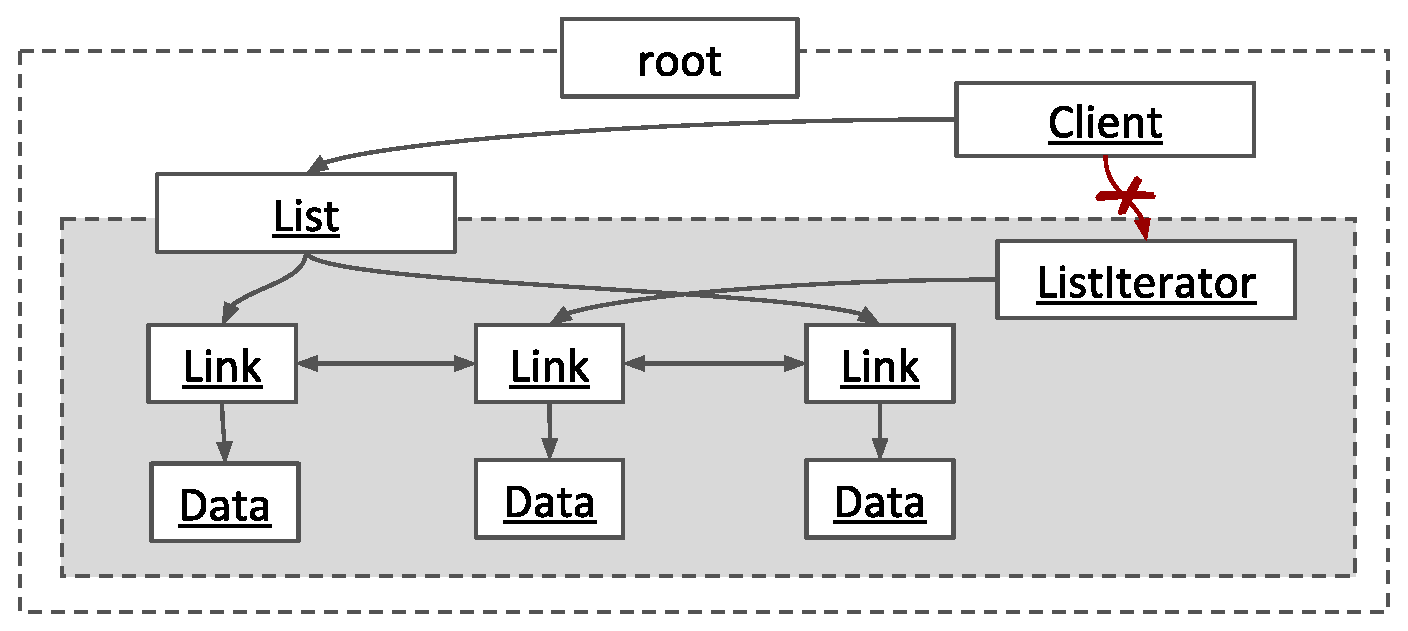
\includegraphics{iterator-fail-inside.eps}
	\caption{List Iterator inside representation}
	\label{fig:iterator-inside}
\end{figure}

\begin{figure}[t]
	\centering
	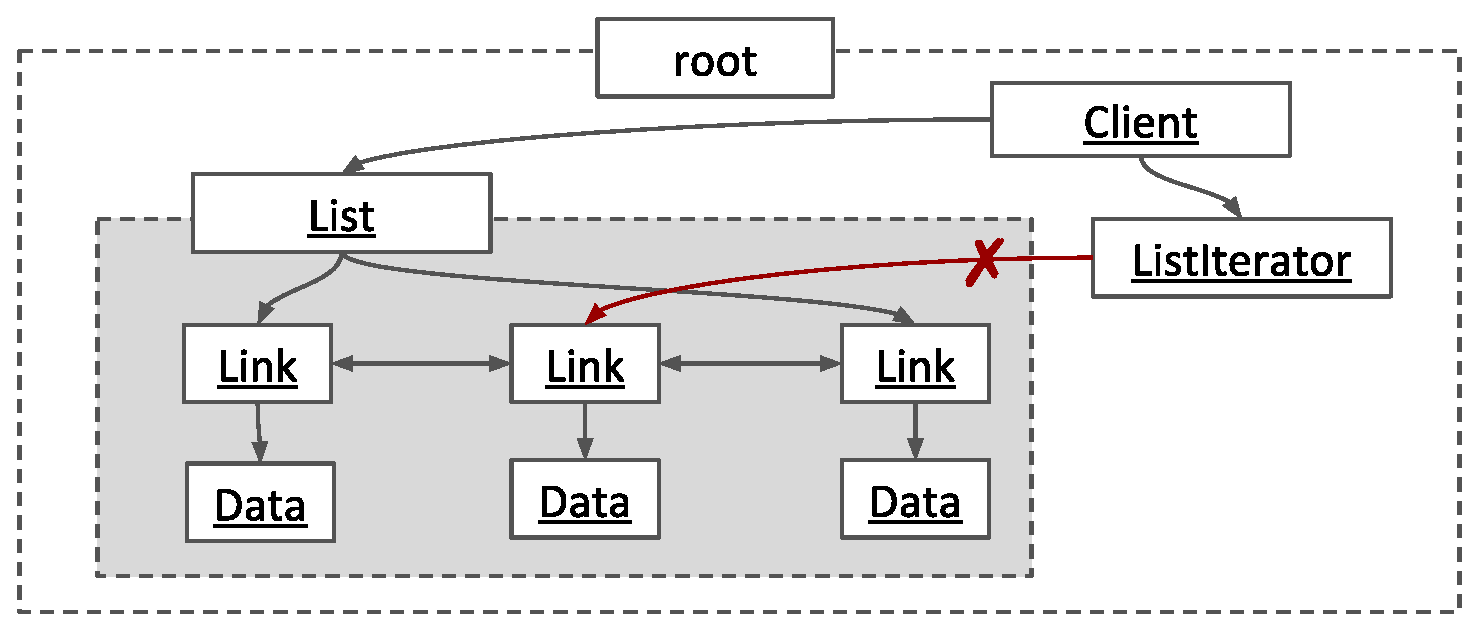
\includegraphics{iterator-fail-outside.eps}
	\caption{List Iterator outside representation}
	\label{fig:iterator-outside}
\end{figure}

\subsection{Binary Operators}
\label{subsec:binary_ops}

Another common operation that is performed regularly in programs is the use of
a binary operator, such as a list append. Sometimes, it is necessary to perform
the binary operation over two values with different owners, such as merging the
results of a parallel reduction function. We have chosen to implement a queue
which allows merging together to simulate this situation.

Once again, the \textbf{owners-as-dominators} discipline is proving to be too
strict to allow such an operation. \Cref{fig:binary-operators} demonstrates
that it is not possible for either object to access each other's representation 
invariants. The \textbf{owners-as-modifiers} discipline will not prevent a
programmer from implementing such an operation.

\begin{figure}[t]
	\centering
	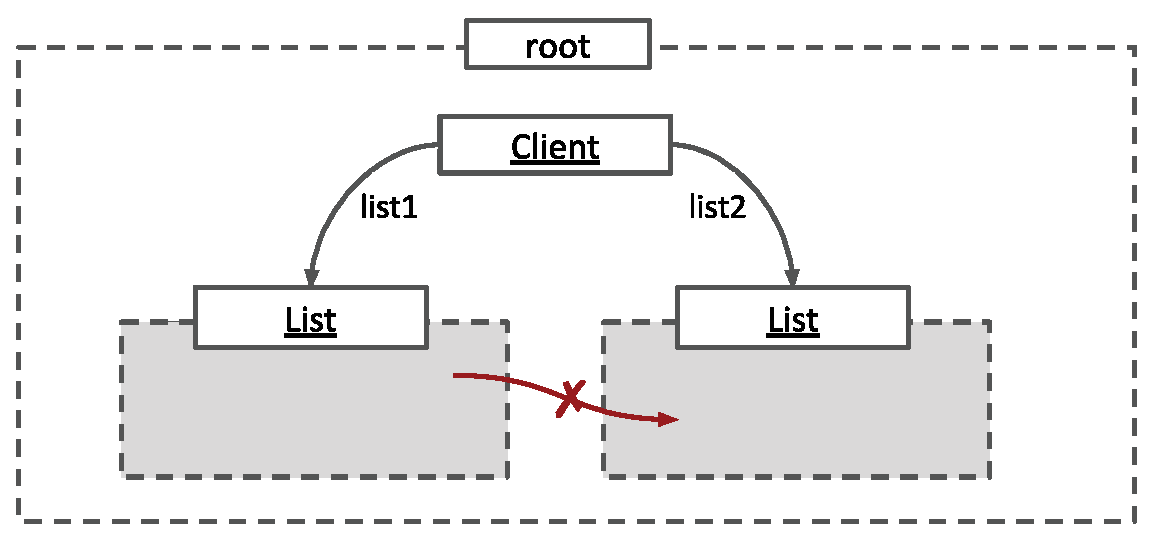
\includegraphics{binary-fail.eps}
	\caption{Binary operators do not have access to another object's 
		representation invariant}
	\label{fig:binary-operators}
\end{figure}

Universe Types allowed objects with a \lstinline|peer| \cite{dietl11gut}
relationship to explore each other's representations. Therefore, binary
operators could be implemented. Even if the binary operator did not have
\lstinline|peer| access, it is possible to implement it with only read-access.
Typically, binary operators do not modify its operands, hence read-only access
is sufficient.

If multiple ownership is allowed, relaxing the \textbf{owners-as-dominators}
discipline, then binary operators can be implemented. This can be accomplished
by declaring the operator as accepting objects that the type has co-ownership
for.



\begin{itemize}

	\item The \textit{Binary Operators} 
	
	\item A number of the examples contain unique features that aren't found in
		more than one type system, for example: multiple ownership, ownership
		transfer, and accommodation of generics. Because they have no analogue
		these features can't be compared. The situation is similar for ownership
		parameters and constraints.

\end{itemize}

\section{Conclusion}
\label{sec:conclusion}

Our exploration of the various type systems here surfaced a number of issues and
caveats which may limit their use or hinder mainstream adoption.

For one, the type systems presented are all pure, static type systems, but the
language that they target, Java, does not have such a type system. Notably Java
has runtime polymorphism, reflective features, and relies on dynamic casts to
cope with certain situations (for example, casting a collection of abstract
objects to subtypes for use). As such, in practice compile-time checking alone
is insufficient \cite{boyapati04safejava} and runtime checks are required,
especially if Java interoperability is a requirement.

Annotations are also a burden on programmers. Ownership
inference~\cite{boyapati04safejava} is possible to an extent but cannot be done
in general, as there are complex ownership scenarios (iterators being the prime
example) that cannot possibly be inferred from source code. The implication is
that programmers will need to provide some amount of annotations. This amount
varies with the various systems, but adds significant cognitive burden due to
the sheer number of new constructs~\cite{boyapati04safejava} or heavily utilise
concepts which are not immediately evident from source
code~\cite{cameron07mojo}. It is also easy to misuse annotations: for example,
trivially letting ownership checks pass by declaring everything as owned by
\lstinline|world|.

In summary, while benefits of ownership types are undeniable and they provide
an unprecedented amount of safety and encapsulation, they can also be cumbersome
to work with. We postulate that they will see most use in safety-critical
applications, where their strengths in ensuring the correctness of programs can
outweigh the costs of using them.

%
% Reference to \cref{code:car_eng_test}, \cref{sec:test} and
% \cref{fig:iterator-inside-test,fig:iterator-outside-test}.
%
% % Citations
% aldrich04domains~\cite{aldrich04domains},\newline
% aldrich02aliasjava~\cite{aldrich02aliasjava},\newline
% almeida97balloons~\cite{almeida97balloons},\newline
% boyapati04safejava~\cite{boyapati04safejava},\newline
% boyapati02races~\cite{boyapati02races},\newline
% boyapati03innerclass~\cite{boyapati03innerclass},\newline
% boyapati03rtsj~\cite{boyapati03rtsj},\newline
% cameron07mojo~\cite{cameron07mojo},\newline
% cameron10encoding~\cite{cameron10encoding},\newline
% clarke03ownership~\cite{clarke03ownership},\newline
% clarke02ownership~\cite{clarke02ownership},\newline
% clarke13aliasing~\cite{clarke13aliasing},\newline
% clarke98ownership~\cite{clarke98ownership},\newline
% cunningham08ut~\cite{cunningham08ut},\newline
% dietl09gut~\cite{dietl09gut},\newline
% dietl11gut~\cite{dietl11gut},\newline
% dietl07gut~\cite{dietl07gut},\newline
% dietl13ownership~\cite{dietl13ownership},\newline
% dietl08dependent~\cite{dietl08dependent},\newline
% dietl05jml~\cite{dietl05jml},\newline
% hogg91islands~\cite{hogg91islands},\newline
% muller02modular~\cite{muller02modular},\newline
% muller99universes~\cite{muller99universes},\newline
% noble98alias~\cite{noble98alias}, \newline
% clarke13survey~\cite{clarke13survey}
%

\nocite{*}

\bibliographystyle{abbrv}
\bibliography{report}

\end{document}
